%---------------------------------------------------------------------
%
%                          Editor
%
%---------------------------------------------------------------------

\chapter{Vision general}

En el cap�tulo anterior, exploramos la naturaleza de un motor de juego y un editor, as� como su interacci�n mutua. Mientras que un motor con un editor puede acelerar significativamente el proceso de desarrollo de juegos, los editores en s� mismos representan una inversi�n considerable en t�rminos de recursos y tiempo. Los editores con motor integrado suelen ser extensos y ofrecen una amplia gama de funcionalidades para atender diversas necesidades de desarrollo de juegos. Sin embargo, esta versatilidad puede ser un inconveniente si se busca crear un juego peque�o y simple, ya que obliga a los desarrolladores a aprender a utilizar caracter�sticas innecesarias y puede resultar en un producto final con un exceso de funcionalidades no utilizadas.

\medskip

Por lo tanto, hemos optado por desarrollar un motor dirigido por datos espec�ficamente dise�ado para juegos 2D simples y eficientes, complementado por un editor que permita la creaci�n de estos juegos. En nuestro enfoque, los datos desempe�an un papel central al servir como el medio de comunicaci�n entre el editor y el motor. El editor genera datos que el motor puede leer e interpretar, permitiendo as� desarrollar un motor especializado en juegos 2D simples y eficientes sin comprometerse con caracter�sticas innecesarias.

\medskip

En nuestro modelo, la entidad fundamental es la escena, que contiene entidades individuales. Estas entidades est�n equipadas con componentes que, a su vez, almacenan atributos que representan datos espec�ficos. Estos atributos pueden variar desde tipos de datos simples hasta referencias a otras entidades o recursos como imagenes. Las referencias a entidades se realiza mediante IDs que tienen asignadas. Los elementos como im�genes, escenas y otros recursos que son representados como archivos se identifican a trav�s de sus nombres de archivo, y se ha implementado una funci�n de manejo de errores que notificar� a los usuarios en caso de que la ubicaci�n de estos archivos se modifique. La serializaci�n de estos datos se lleva a cabo en formato JSON, lo que permite una representaci�n eficiente y legible de los objetos del juego.

\medskip

Una decisi�n cr�tica en nuestro proyecto fue mantener el motor y el editor como entidades separadas en lugar de integrarlos. Esto nos otorga la flexibilidad de utilizar el motor y el editor con otros sistemas si fuera necesario, con la condici�n de establecer una forma coherente de transferir informaci�n entre ellos. Esta independencia de un motor de juego espec�fico nos brinda la libertad de elegir el motor m�s adecuado para las necesidades particulares de nuestro proyecto, un aspecto esencial cuando se trata de proyectos altamente personalizados.

\medskip

TODO:------------------------------------------
   Se decide tirar por un lenguaje visual porque el objetivo, como se dijo en el cap�tulo 1, era que pudieran usarlo no programadores. Vale, esta decisi�n �que nos supone a vista de p�jaro, que es donde estamos ahora? Hay que ver qu� queremos soportar porque hay que serializarlo/deserializarlo, crear el editor, y crear la "m�quina virtual". Adem�s hay que ver c�mo se va a hacer "el puente" para que desde un dibujo (programa visual) se pueda llamar a un m�todo de C++ del motor y al rev�s, sea cual sea. Y �vamos a usar eventos o update? Habr� que decidir qu� eventos vamos a tener, c�mo vamos a "dispararlos" desde el motor al gameplay y c�mo vamos a "pintar" la reacci�n a un evento en el "c�digo".


% \begin{figure}[h]
%     \centering
%     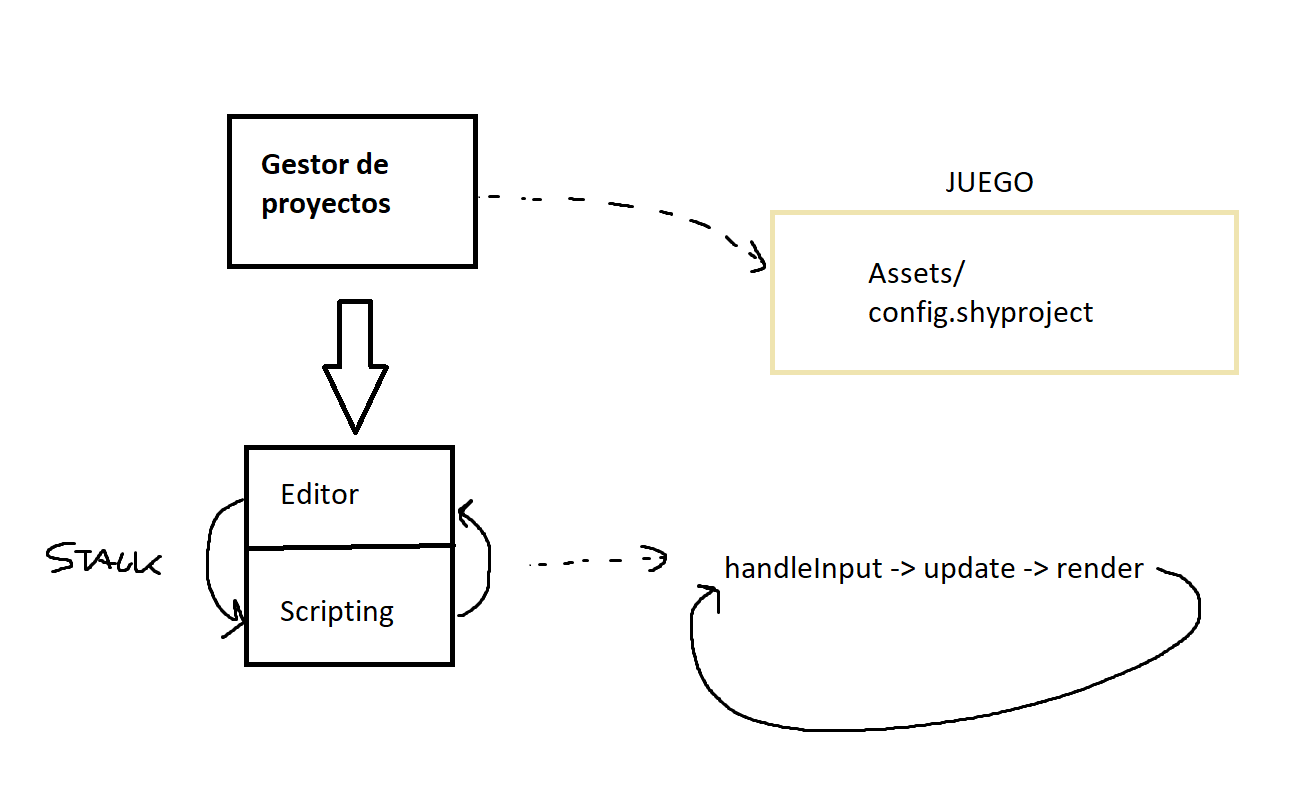
\includegraphics[width=0.6\textwidth]{Imagenes/Vectorial/FuncionamientoEditor.png}
%     \caption{Flujo de funcionamiento del editor.}
%     \label{fig:funcionamientoEditor}
% \end{figure}

%------------------------------------------------  --------------------------------------------


